\documentclass[11pt]{article}

\setlength{\topmargin}{0.0in}
\setlength{\oddsidemargin}{0.0in}
\setlength{\evensidemargin}{0.0in}
\setlength{\rightmargin}{1.0in}
\setlength{\headheight}{0in}
\setlength{\textwidth}{6.5in}
\setlength{\textheight}{9in}
\setlength{\footskip}{0.5in}
\setlength{\parskip}{0.75em}
\setlength{\parindent}{0in}
\setlength{\voffset}{-0.5in}
\usepackage{graphicx}
\usepackage{amsmath,amssymb}
\usepackage{listings}
\lstset{basicstyle=\ttfamily\small,columns=fullflexible,keepspaces=true}
\usepackage{xcolor}
\usepackage{enumitem}
\usepackage{algorithm}
\usepackage{algpseudocode}
\usepackage{amsmath}
\usepackage{float}

\newcommand{\logit}{\operatorname{logit}}
\widowpenalty=10000
\clubpenalty=10000

\begin{document}

\framebox{\begin{minipage}{1.0 \textwidth}
\textit{Computational Methods for Biological Modeling and Simulation (02512/02712)}

\textbf{Name:Jeffrey Wang}

\textbf{Andrew ID:jdw2}

\textbf{AI use statement:}
Improve tricky phrasing when describing reasoning.\\
Reinterpreting question to better understand it.\\
Convert text into latex when there's too many variable involved.
\end{minipage}}

\begin{center}
{\huge Problem Set 2 }\\
\end{center}

Released Thursday, September 24. Due Thursday, October 8 at 11:59pm.
Programming problems must use Python with the standard library only.
Starred problems are only for 02-712 students.

{\bf Problem 1 (15 points):} Suppose we are looking for serum biomarkers
that predict early risk of pancreatic cancer.  We want to take a blood
sample, measure the levels of two candidate proteins, A and B, and use them
to predict whether the person is likely to develop cancer.  The table shows
the levels of both proteins in eight people and whether each person was
later found to have pancreatic cancer.

\begin{center}
\begin{tabular}{|c|c|c|}
\hline
Protein A & Protein B & Cancer\\
\hline
1.3 & 2.5 & N\\
2.4 & 8.4 & Y\\
1.4 & 0.2 & N\\
2.6 & 9.6 & N\\
4.9 & 4.1 & Y\\
3.1 & 6.1 & Y\\
2.5 & 3.2 & N\\
0.1 & 2.1 & N\\
\hline
\end{tabular}
\end{center}

a. (2 points) Estimate the mean and variance of protein A and of protein B. Use the sample variance, dividing by $n-1$.

\textcolor{red}{%
$\mu_A = \frac{1.3 + 2.4 + 1.4 + 2.6 + 4.9 + 3.1 + 2.5 + 0.1}{8} \approx 2.288$\\
$s^2_A = \frac{(1.3 - 2.288)^2 + (2.4 - 2.288)^2 + (1.4 - 2.288)^2 + (2.6 - 2.288)^2 + (4.9 - 2.288)^2 + (3.1 - 2.288)^2 + (2.5 - 2.288)^2 + (0.1 - 2.288)^2}{8-1} \approx \frac{14.189}{7} = 2.0270$\\
$\mu_B = \frac{2.5 + 8.4 + 0.2 + 9.6 + 4.1 + 6.1 + 3.2 + 2.1}{8} = 4.525$\\
$s^2_B = \frac{(2.5 - 4.525)^2 + (8.4 - 4.525)^2 + (0.2 - 4.525)^2 + (9.6 - 4.525)^2 + (4.1 - 4.525)^2 + (6.1 - 4.525)^2 + (3.2 - 4.525)^2 + (2.1 - 4.525)^2}{8-1} = \frac{73.875}{7} \approx 10.554$\\
}

b. (2 points) Estimate the covariance of the levels of proteins A and B, again dividing by $n-1$.

\textcolor{red}{
$\texttt{Cov}(A, B) = \frac{(A_1 - \mu_A)(B_1 - \mu_B) + \ldots + (A_n - \mu_A)(B_n - \mu_B)}{n-1} = \frac{13.0525}{7} \approx 1.865$
}

c. (3 points) Estimate the probability that both protein levels are above 2, and the probability that protein A is above 2 given that protein B is above 2.

\textcolor{red}{
$P(A_i > 2 \cup B > 2) = \frac{5}{8} = 0.625$\\
$P(A_i > 2 | B > 2) = \frac{5}{7} \approx 0.714$
}

d. (3 points) Suppose the test is called positive when both protein levels are at least 2.5.  Estimate the false positive rate, the probability of a positive test for a person who does not develop cancer, and the false negative rate, the probability of a negative test for a person who does develop cancer.

\textcolor{red}{
$\texttt{FPR} = \frac{2}{5} = 0.40$\\
$\texttt{FNR} = \frac{1}{3} \approx 0.333$
}

e. (5 points) A larger study finds a false positive rate of 5\% and a false negative rate of 20\%, and 1\% of the population develops pancreatic cancer. Use Bayes' rule to find the probability that a person develops cancer given a positive test, and given a negative test.  In a sentence, explain why the first probability is so much smaller than the test's sensitivity, the 80\% probability of a positive test for a person who develops cancer.

\textcolor{red}{
$P(C|P) = \frac{P(P|C) P(C)}{P(P)}$\\
$P(P|C) = 1 - 0.20 = 0.80$\\
$P(P|\neg C) = 0.20$\\
$P(P) = P(P|C)P(C) + P(P|\neg C)P(\neg C) = (0.80)(0.01) + (0.05)(0.99) = 0.0575$\\
$P(C|P) = \frac{P(P|C) P(C)}{P(P)} = \frac{(0.80)(0.01)}{(0.0575)} \approx 0.139$\\
\\
$P(C|N) = \frac{P(N|C) P(C)}{P(N)}$\\
$P(N|C) = 0.20$\\
$P(N|\neg C) = 1 - 0.05 = 0.95$\\
$P(N) = P(N|C)P(C) + P(N|\neg C)P(\neg C) = (0.20)(0.01) + (0.95)(0.99) \approx 0.943$\\
$P(C|N) = \frac{P(N|C) P(C)}{P(N)} = \frac{(0.20)(0.01)}{(0.943)} \approx 0.00212$\\
\\
The probability that a person develops cancer given a positive test (13.9\%) is so much smaller than the test's sensitivity (80\%) because due to 1\% of the population developing pancreatic cancer, the number of false positives you might get can be much greater than true positives.
}

{\bf Problem 2 (20 points):} A research group uses a large language model to screen the literature for papers that report a particular drug interaction. The model flags 500 papers as relevant.  The group chooses 20 of the flagged papers uniformly at random, without replacement, and reads them carefully. Eighteen of the 20 are relevant.  Let $K$ be the unknown number of relevant papers among the 500 flagged papers.  Assume the careful reading is always correct.

a. (3 points) Write the probability of observing $y$ relevant papers in the sample of 20, given $K$.  Name the distribution.

\textcolor{red}{
$P(y | K) = \frac{\binom{K}{y} \binom{500 - K}{20 - y}}{\binom{500}{20}}$
}

b. (3 points) Put a uniform prior on $K\in\{0,1,\ldots,500\}$.  Write the posterior distribution of $K$ up to a normalizing constant.  Which values of $K$ have posterior probability zero, and why?

\textcolor{red}{
$P(K | y = 18) \propto \binom{K}{18} \binom{500 - K}{2}$\\
Because the researchers found that of the 20 flagged papers chosen, only 18 of them were relevant and 2 were irrelevant, of the 500 total papers, there must be $\ge 18$ relevant papers but also $\le 500-2$ relevant papers. Thus, any value of $K < 18 \lor K > 498$ will have a posterior probability of 0.
}

c. (5 points) Write a program that computes the normalized posterior for every $K$.  Report the posterior mode, the posterior mean, and a 90\% central interval $[K_{\rm lo},K_{\rm hi}]$, where $K_{\rm lo}$ is the smallest $k$ with $P(K\le k\mid y)\ge0.05$ and $K_{\rm hi}$ is the smallest $k$ with $P(K\le k\mid y)\ge0.95$.  The binomial coefficients are large, so use exact integers (as Python's {\tt math.comb} does) or work with logarithms.  Include your code.

\textcolor{red}{
Posterior mode: $450$\\
Posterior mean: $432.545$\\
$90\%$ CI: $[367,\ 480]$
}

d. (5 points) Now suppose the group believes the model has some precision $\theta$, the probability that a flagged paper is relevant, and models $K\mid\theta\sim\mathrm{Binomial}(500,\theta)$ with $\theta\sim\mathrm{Beta}(a,b)$, whose density is proportional to $\theta^{a-1}(1-\theta)^{b-1}$ on $(0,1)$, with $a,b>0$. Under this model, given $\theta$, each of the 500 flagged papers is relevant independently with probability $\theta$. You may use two facts. First,
\[
\int_0^1\theta^k(1-\theta)^{n-k}\,d\theta=\frac{k!\,(n-k)!}{(n+1)!}.
\]
Second, if $\theta\sim\mathrm{Beta}(a,b)$ and we observe $r$ successes and $f$ failures in independent Bernoulli($\theta$) trials, then the posterior distribution of $\theta$ is Beta$(a+r,b+f)$, with mean $(a+r)/(a+b+r+f)$.
(i) Show that with $a=b=1$ the implied prior on $K$ is uniform, the prior of part (b).  (ii) Write the posterior mean of $K$ as a
formula in $a$ and $b$.  (Hint: $K$ is 18 plus the number of
relevant papers among the 480 unread ones, and given $\theta$ that number has expected value $480\theta$.)  Evaluate it for a prior of Beta(9, 1) and for a prior of Beta(2, 8), and explain the difference in one or two sentences.
\textcolor{red}{
\begin{enumerate}[label=(\roman*)]
    \item 
        Because $a=b=1, P(\theta) = \theta^{1-1}(1-\theta)^{1-1} = 1$. Thus,\\
        $P(K) = \int_0^1 P(K\vert{}\theta)P(\theta) d\theta \\
        = \int_0^1 \binom{500}{K} \theta^K (1-\theta)^{500-K} (1) d\theta\\
        = \frac{500!}{K!(500-K)!} \frac{K!(500-K)!}{501!} = \frac{1}{501}$\\
        The implied prior on $K$ is uniform.
    \item 
        $E[K|y] = 18 + 480 \cdot \left(\frac{a+18}{a+18+b+2} \right) = 18 + 480 \cdot \left(\frac{a+1}{a+b+20}\right)$\\
        Prior of Beta(9, 1): $E[K|y] = 18 + 480 \cdot \left(\frac{9+18}{9+1+20} \right) = 450$\\
        Prior of Beta(2, 8): $E[K|y] = 18 + 480 \cdot \left(\frac{2+18}{2+8+20} \right) = 338$\\
        The difference is a result of $a$ corresponding to the prior weight given to relevant papers and $b$ to irrelevant papers. In Beta(9, 1), our assumption is that the model's precision is around 90\% contrasting to Beta(2, 8) where we assume the model has a poor accuracy. These are then reflected in the posterior means of $K$ in each prior.
\end{enumerate}
}

e. (4 points) The group wants to know how many relevant papers exist in the entire literature, not just among the flagged papers.  What can this design not tell them?  Describe a change to the design, and the extra quantity your model would need, to answer that question.

\textcolor{red}{
This design cannot tell them the false negatives or relevant papers not flagged. If we wanted to answer this question, a change to the design might look like randomly sampling the unflagged papers to deduce if they're relevant or not so we can have a \texttt{FNR}. The model would thus need to know the total number of un-flagged papers.
}

{\bf Problem 3 (15 points):} We want to interpret a noisy image by writing a generative model for it.  The data are an $n\times n$ array $M$ of pixel intensities $m_{ij}$, with the background intensity already subtracted.  A pixel inside a bright object has intensity drawn from $\mathcal N(1,1)$, and a background pixel has intensity drawn from $\mathcal N(0,1)$, independently across pixels given the objects.  Objects are squares aligned with the pixel grid.  For each part, write the generative process in order, state which quantities are unknown, and write the joint probability of the unknowns and the data $M$.  You do not need to say how you would fit the model.

a. (3 points) The image contains exactly one object of known size $k\times k$.  Its upper-left corner is equally likely to be at any position that keeps the whole object inside the image.

\textcolor{red}{
Let $S$ be the set of pixels covered by an object. $P(M|S)$ would represent the likelihood of the observed data/image $M$ given set $S$ consisting of pixels covered by objects. Because pixel intensities are drawn independently once the objects are placed, the joint probability of image $M$ would be the product of probabilities of every pixel. Thus, what constitutes the foreground pixels would be for any pixel $x=(i,j) \in S$, intensity $m_{ij}$ is sampled from $\mathcal N(1,1)$ which applies a standard Gaussian probability density function centered at 1 to those pixels. The background pixels would be for any pixel $x=(i,j) \notin S$, intensity $m_{ij}$ is sampled from $\mathcal N(0,1)$.\\
\\
Offloading my interpretation out of the way, if $M$ is one object of known size $k \times k$...
\begin{enumerate}
    \item \textbf{Generative Process:}\\
        \begin{enumerate}
            \item 
                First, uniformly draw the top left of the object $(u,v)$ for valid $u,v$ that land in $(n-k+1)^2$.
            \item 
                Second, determine pixels covered by the object and put into set $S$.
            \item 
                Third, draw pixel intensities
                \[
                m_{ij} = 
                \begin{cases} 
                      \mathcal N(1,1) & (i,j) \in S \\
                      \mathcal N(0,1) & (i,j) \notin S 
                \end{cases}
                \]
        \end{enumerate}
    \item \textbf{Unknown Quantities:}\\
        We don't know which pixels fall under the object's location. We only see the final, noisy, observed data $D$ so the coordinate of the pixel in the top left of the object $(u,v)$ is the hidden parameter.
    \item \textbf{Joint Probability:}\\
        $P(M, u, v) = \frac{1}{(n-k+1)^2} P(M|S)$
\end{enumerate}
}

b. (3 points) The size $k$ is now unknown, with prior probability uniform on $\{1,\ldots,k_{\max}\}$ for a known $k_{\max}\le n$.

\textcolor{red}{
\begin{enumerate}
    \item \textbf{Generative Process:}\\
        \begin{enumerate}
            \item 
                First, uniformly draw $k$ from $\{1,\ldots,k_{\max}\}$.
            \item 
                Second, uniformly draw the top left of the object $(u,v)$ for valid $u,v$ that land in $(n-k+1)^2$.
            \item 
                Third, determine pixels covered by the object and put into set $S$.
            \item 
                Fourth, draw pixel intensities
                \[
                m_{ij} = 
                \begin{cases} 
                      \mathcal N(1,1) & (i,j) \in S \\
                      \mathcal N(0,1) & (i,j) \notin S 
                \end{cases}
                \]
        \end{enumerate}
    \item \textbf{Unknown Quantities:}\\
        Now we don't know size $k$ and the top-left pixel of the object $(u,v)$.
    \item \textbf{Joint Probability:}\\
        $P(M, k, u, v) = \frac{1}{k_{max}} \frac{1}{(n-k+1)^2} P(M|S)$
\end{enumerate}
}

c. (4 points) The image now contains an unknown number $s\ge0$ of objects, all of the same unknown size $k$, with the prior on $k$ from part (b).  The prior on $s$ is geometric, $P(s)=\rho(1 \rho)^s$ for $s=0,1,2,\ldots$ and known $0<\rho<1$, independently of $k$.  Given $k$ and $s$, the corners are independent and uniform as in part (a).  Label the objects $1,\ldots,s$ in the order they are drawn.  Objects may overlap, and a pixel covered by any object has mean 1.

\textcolor{red}{
\begin{enumerate}
    \item \textbf{Generative Process:}\\
        \begin{enumerate}
            \item 
                First, uniformly draw $k$ from $\{1,\ldots,k_{\max}\}$.
            \item 
                Second, draw $s$ from $P(s)=\rho(1 \rho)^s$.
            \item 
                Third, for every object $o \in \{1,\ldots,s\}$, uniformly draw the top left of the object $(u_o,v_o)$ for valid $u_o,v_o$ that land in $(n-k+1)^2$.
            \item 
                Fourth, determine pixels covered by the $s$ objects and put into set $S$.
            \item 
                Fifth, draw pixel intensities
                \[
                m_{ij} = 
                \begin{cases} 
                      \mathcal N(1,1) & (i,j) \in S \\
                      \mathcal N(0,1) & (i,j) \notin S 
                \end{cases}
                \]
        \end{enumerate}
    \item \textbf{Unknown Quantities:}\\
        Now we don't know the number of objects $s$, size $k$, and the top-left pixel of each object $(u_o,v_o),\ o \in \{1,\ldots,s\}$.
    \item \textbf{Joint Probability:}\\
        $P(M, s, k, \{(u_o, v_o)\}) = (\rho(1-\rho)^s)\frac{1}{k_{max}} \frac{1}{\prod_{o=1}^{s}(n-k+1)^2} P(M|S) \forall o \in \{1,\ldots,s\}$
\end{enumerate}
}

d. (5 points) Now each object $c$ has its own size $k_c$, drawn
independently with probability proportional to $q(1-q)^{k_c-1}$ for $k_c=1,\ldots,n$, where $0<q<1$ is known.  This is a geometric distribution truncated so the object fits in the image.  Draw $s$ as in part (c), then draw the corners independently and uniformly given their respective sizes. Write the joint probability, and list which quantities are drawn once per image, once per object, and once per pixel.

\textcolor{red}{
\begin{enumerate}
    \item \textbf{Generative Process:}\\
        \begin{enumerate}
            \item 
                First, uniformly draw $k$ from $\{1,\ldots,k_{\max}\}$.
            \item 
                Second, draw $s$ from $P(s)=\rho(1 \rho)^s$.
            \item 
                Third, for every object $o \in \{1,\ldots,s\}$, geometrically with known $0 < q < 1$ draw $k_o$ from $\{1,\ldots,n\}$.
            \item 
                Fourth, for every object $o \in \{1,\ldots,s\}$, uniformly draw the top left of the object $(u_o,v_o)$ for valid $u_o,v_o$ that land in $(n-k_o+1)^2$.
            \item 
                Fifth, determine pixels covered by the $s$ objects and put into set $S$.
            \item 
                Sixth, draw pixel intensities
                \[
                m_{ij} = 
                \begin{cases} 
                      \mathcal N(1,1) & (i,j) \in S \\
                      \mathcal N(0,1) & (i,j) \notin S 
                \end{cases}
                \]
        \end{enumerate}
    \item \textbf{Unknown Quantities:}\\
        Now we don't know the number of objects $s$, each of their size $k_o \forall o \in \{1,\ldots,s\}$, and the top-left pixel of each object $(u_o,v_o) \forall o \in \{1,\ldots,s\}$.
    \item \textbf{Joint Probability:}\\
        $P(M, s, \{k_o\}, \{(u_o, v_o)\}) = (\rho(1-\rho)^s)z \prod_{o=1}^{s} \left(\frac{q(1-q)^{k_o-1}}{\sum_{i=1}^n q(1-q)^{i-1}} \frac{1}{(n-k+1)^2} \right) P(M|S) \forall o \in \{1,\ldots,s\}$
\end{enumerate}
}

{\bf Problem 4 (15 points):} A lytic phage infects a bacterium and, after a delay, bursts the cell.  The times from infection to lysis, in minutes, for six infected cells are 1.8, 14, 6.5, 10, 8.1 and 0.28. Assume the times are independent across cells.

The likelihood of a parameter value is the probability density of the observed data under that value, viewed as a function of the parameter. For independent observations it is the product of their densities.  It is usually easier to work with its logarithm, the log-likelihood, which turns the product into a sum.  The maximum likelihood estimate (MLE) is the parameter value with the largest likelihood.  For a single parameter, setting the derivative of the log-likelihood to zero gives candidates in the interior of the parameter space. A negative second derivative confirms a local maximum; also check whether other candidates or boundary values give a larger likelihood.

a. (2 points) Compute the sample mean and sample standard deviation.

\textcolor{red}{
$\bar{t} = \frac{1.8 + 14 + 6.5 + 10 + 8.1 + 0.28}{6} = \frac{40.68}{6} = 6.78$\\
$s^2 = \frac{(-4.98)^2 + (7.22)^2 + (-0.28)^2 + (3.22)^2 + (1.32)^2 + (-6.5)^2}{6-1} = \frac{131.368}{5} \approx 26.274$\\
$s = \sqrt{26.274} \approx 5.126$
}

b. (4 points) Suppose lysis is a single random event occurring at constant rate $\lambda$, so each time is exponential with density
$\lambda e^{-\lambda t}$.  Write the log-likelihood of the six times and derive the maximum likelihood estimate of $\lambda$.  Evaluate it.

\textcolor{red}{
$\ell(\lambda) = \sum_{i=1}^n \ln(\lambda e^{-\lambda t_i}) = n \ln(\lambda) - \lambda \sum_{i=1}^n t_i$\\
$\frac{d\ell}{d\lambda} = \frac{n}{\lambda} - \sum t_i = 0\\
\hat{\lambda} = \frac{n}{\sum t_i} = \frac{6}{40.68} \approx 0.147$
}

c. (4 points) Suppose instead lysis requires two independent sequential steps, each exponential with the same rate $\lambda$, so the time has density $\lambda^2 t e^{-\lambda t}$.  Derive the maximum likelihood estimate of $\lambda$ and evaluate it.

\textcolor{red}{
$\ell(\lambda) = \sum_{i=1}^n \ln(\lambda^2 t_i e^{-\lambda t_i}) = 2n \ln(\lambda) + \sum_{i=1}^n \ln(t_i) - \lambda \sum_{i=1}^n t_i$\\
$\frac{d\ell}{d\lambda} = \frac{2n}{\lambda} - \sum t_i = 0\\
\hat{\lambda} = \frac{2n}{\sum t_i} = \frac{12}{40.68} \approx 0.295$
}

d. (3 points) Evaluate each model's likelihood at its maximum likelihood estimate.  Which model fits these data better, and what feature of the data explains it?

\textcolor{red}{
\textbf{a.} $\ell(0.147) = 6 \ln(0.147) - 0.147(40.68) \approx -17.484$\\
\textbf{b.} $\ell(0.295) = 12 \ln(0.295) + \ln(1.8 \times 14 \times 6.5 \times 10 \times 8.1 \times 0.28) - 0.295(40.68) \approx -18.430$\\
The model from (a) involving a single random event fits the data better because it has a higher log-likelihood because the observed lysis times are pretty short. The model from (b) involving two independent steps intuitively requires an initial event before a burst can occur and mathematically this is supported because $f(t) = \lambda^2 t e^{-\lambda t}$ will be $0$ if $t=0$. The single random event model doesn't have this and enables a higher probability of a cell immediately bursting.
}

e. (2 points) For the one-step model, put an exponential prior with rate 1 on $\lambda$.  Derive the MAP estimate and compare it with part (b).

\textcolor{red}{
$p(\lambda | t) \propto \left( \lambda^n e^{-\lambda \sum t_i} \right) e^{-\lambda} = \lambda^n e^{-\lambda (\sum t_i + 1)}$\\
$\ln(p(\lambda | t)) = n\ln(\lambda) + \lambda (\sum_{i=1}^n t_i + 1)$\\
$\frac{d}{d\lambda} = \frac{n}{\lambda} - \left(\sum_{i=1}^n t_i + 1\right) = 0\\
\lambda_{MAP} = \frac{n}{\sum_{i=1}^n t_i + 1} = \frac{6}{40.68 + 1} = 0.144$\\
The MAP estimate is lower than the MLE and this makes sense because in formula for $\lambda_{MAP}$, the prior adds 1 to the denominator versus the MLE is built off a prior assumption that heavily favors smaller values for the rate.
}

{\bf Problem 5 (20 points):} A protein is localized along the long axis of a polarized cell.  Scaling the axis to $[0,1]$, the position $x$ of a molecule has density
\[
f(x)=c\,x\sin(\pi x),\qquad 0\le x\le1.
\]
We want to generate random positions to place molecules in simulated cell images.  Assume you can draw independent $U[0,1]$ samples.

Two standard methods turn uniform draws into draws from $f$.  The inverse transformation method draws $u\sim U[0,1]$ and returns the $x$ that solves $F(x)=u$, where $F$ is the cumulative distribution function of $f$.  The result has density $f$, because $P(X\le x)=P(U\le F(x))=F(x)$.  Rejection sampling instead uses an envelope, a density $g$ that we can already sample, together with a constant $M$, such that $f(x)\le Mg(x)$ for every $x$.  We draw a proposal $x$ from $g$ and an independent $v\sim U[0,1]$.  We accept $x$ if $vMg(x)\le f(x)$, and otherwise we discard it and draw again.  The accepted values have density $f$.  Each proposal is accepted with probability $1/M$, so an envelope that fits $f$ more closely wastes fewer draws.

a. (2 points) Find the normalizing constant $c$.

\textcolor{red}{
$\int_0^1 c x \sin(\pi x) dx = 1\\
= c \cdot \left[ -\frac{x}{\pi}\cos(\pi x) \right]_0^1 - \int_0^1 \left(-\frac{1}{\pi}\cos(\pi x)\right) dx\\
= c \left( \frac{1}{\pi} \right) = 1\\
c = \pi
$
}

b. (3 points) Derive the cumulative distribution function $F(x)$ and check that $F(1)=1$.

\textcolor{red}{
$F(x) = \int_0^x \pi t \sin(\pi t) dt\\
= \pi \cdot \left[ -\frac{t}{\pi}\cos(\pi t) + \frac{1}{\pi^2}\sin(\pi t) \right]_0^x\\
= \frac{1}{\pi}\sin(\pi x) - x\cos(\pi x)$\\
$F(1) = \frac{1}{\pi}\sin(\pi) - 1\cos(\pi) = 0 - (-1) = 1$
}

c. (4 points) $F$ cannot be inverted in closed form, but we can solve $F(x)=u$ numerically by bisection.  Because $F$ increases from $F(0)=0$ to $F(1)=1$, the solution lies in the interval $[\ell,r]=[0,1]$. Each step evaluates $F$ at the midpoint $m=(\ell+r)/2$.  If $F(m)<u$, the solution lies to the right of $m$, so we set $\ell=m$; otherwise we set $r=m$.  The interval still contains the solution and is half as long, so after $k$ steps any point in it is within $2^{-k}$ of the solution.  (i) Carry out three bisection steps by hand for $u=0.5$, giving the interval after each step. (ii) Using the bound $2^{-k}$ for an arbitrary point in the final interval, how many steps guarantee an error of at most $10^{-6}$?
\textcolor{red}{
\begin{enumerate}[label=(\roman*)]
    \item 
        \begin{enumerate}
            \item 
                $m = 0.5$\\
                $F(0.5) = \frac{1}{\pi}\sin(\pi/2) - 0.5\cos(\pi/2) = \frac{1}{\pi}(1) - 0 \\
                \approx 0.318$.
            \item 
                $m = 0.75$ because $F(0.5) < 0.5$ so move right.\\
                $F(0.75) = \frac{1}{\pi}\sin(3\pi/4) - 0.75\cos(3\pi/4) = \frac{1}{\pi}\left(\frac{\sqrt{2}}{2}\right) - 0.75\left(-\frac{\sqrt{2}}{2}\right) \\
                \approx 0.225 + 0.530 = 0.755$.
            \item 
                $m = 0.625$ because $F(0.75) > 0.5$ so move left.\\
                $F(0.625) = \frac{1}{\pi}\sin(5\pi/8) - 0.625\cos(5\pi/8) \approx \frac{1}{\pi}(0.924) - 0.625(-0.383) \\
                \approx 0.294 + 0.239 = 0.533$.
        \end{enumerate}
    \item 
        $2^{-k} \le 10^{-6}\\
        -k \log_{10}(2) \le -6\\
        k \ge \frac{6}{\log_{10}(2)} \approx 19.932$ steps
\end{enumerate}
}

d. (4 points) Now use rejection sampling with the uniform density $g(x)=1$ on $[0,1]$, so the envelope $Mg$ is a constant of height $M$.  What is the smallest valid $M$?  (Finding the maximum of $f$ requires solving an equation numerically; you may use bisection as in part (c), applied to $f'$ on $[0.5,1]$ and keeping the half of the interval on which $f'$ changes sign.)  Give pseudocode using only $U[0,1]$ draws, and the fraction of proposals accepted.

\textcolor{red}{
Max of $f(x)$ requires solving $f'(x) = \pi\sin(\pi x) + \pi^2 x \cos(\pi x) = 0 \rightarrow \tan(\pi x) = -\pi x \rightarrow x \approx 0.646$\\
$M = f(0.646) \approx 1.818$\\
The fraction of proposals accepted will be $\frac{1}{M} = \frac{1}{1.818} \approx 0.550$\\
Pseudoscope might look like:\\
\begin{algorithm}[H]
\caption{Rejection Sampling Loop}
    \begin{algorithmic}[1]
        \Loop
            \State Draw $x \sim U[0, 1]$
            \State Draw $v \sim U[0, 1]$
            \If{$(1.818v) \le (\pi x \sin(\pi \times x))$}
                \State \Return $x$
            \EndIf
        \EndLoop
    \end{algorithmic}
\end{algorithm}
}

e. (3 points) Two other envelopes are available: $g_1(x)=2x$, which you can sample as $\sqrt{u}$, and $g_2(x)=\frac{\pi}{2}\sin(\pi x)$, which you can sample as $\arccos(1-2u)/\pi$.  For each, find the smallest constant $M$ with $f\le Mg$ and the acceptance fraction.  Which of the three envelopes would you use?
\textcolor{red}{
\begin{enumerate}
    \item $g_1(x) = 2x$\\
    $\pi x \sin(\pi x) \le M (2x)\\
    \frac{\pi}{2} \sin(\pi x) \le M$\\
    $M = \frac{\pi}{2} \texttt{max}\{\sin(\pi x)\}\\
    = \frac{\pi}{2} \texttt{max}\{\sin(\frac{\pi}{2})\} = \frac{\pi}{2} \approx 1.571$\\
    $\frac{1}{M} = \frac{2}{\pi} \approx 0.637$
    \item $g_2(x)=\frac{\pi}{2}\sin(\pi x)$\\
    $\pi x \sin(\pi x) \le M \left(\frac{\pi}{2}\sin(\pi x)\right)\\
    2x \le M$\\
    $M = 2$\\
    $\frac{1}{M} = \frac{1}{2} = 0.5$\\
\end{enumerate}
$g_1(x)$ has a higher acceptance fraction so we reject fewer samples.
}

f. (4 points) Implement the bisection sampler from part (c), stopping after 20 steps and returning the midpoint of the final interval, and the rejection sampler with envelope $g_1$.  Draw $10^5$ samples with each and compare their sample means with the exact mean $1-4/\pi^2\approx0.5947$. Report the observed acceptance fraction of the rejection sampler. Include your code.

\textcolor{red}{
Exact Mean: 0.595\\
Bisection Sample Mean: 0.594\\
Rejection Sample Mean: 0.595\\
Observed Acceptance Fraction: 0.638\\
It seems like both means of the samplers are very close to the hypothetical exact mean which means they are working as intended with an observed acceptance fraction that follows what we got for $g_1$.
}

{\bf *Problem 6 (15 points):} In a GLM with a logit link, a normal prior on the log-odds implies a distribution for the probability itself.  This problem uses the fundamental transformation law to find that distribution. The law says that if $x$ has density $f$ and $y=\phi(x)$, where $\phi$ is continuously differentiable and strictly monotone with $\phi'(x)\ne0$, then $y$ has density
\[
g(y)=f(x)\left|\frac{dx}{dy}\right|,\qquad x=\phi^{-1}(y).
\]
The factor $|dx/dy|$ corrects for how $\phi$ stretches or compresses intervals, since probability is conserved while lengths change.  Let $a\sim\mathcal N(0,1)$.

a. (3 points) Let $\eta=m+s\,a$ with $s>0$.  Find the density of $\eta$.

\textcolor{red}{
$\eta = m+sa \rightarrow a = \frac{\eta - m}{s}\\
\frac{da}{d\eta} = \frac{1}{s}\\
g(\eta) = f\left(\frac{\eta - m}{s}\right) \left\vert{} \frac{1}{s} \right\vert{} = \frac{1}{\sqrt{2\pi s^2}} e^{-\frac{(\eta - m)^2}{2s^2}}$
}

b. (4 points) Let $p=1/(1+e^{-\eta})$, with $\eta$ from part (a).  Find the density of $p$ on $(0,1)$.

\textcolor{red}{
$p = 1 / (1 + e^{-\eta}) \rightarrow \eta = \ln\left(\frac{p}{1-p}\right)\\
\frac{d\eta}{dp} = \frac{1}{p(1-p)}\\
g(p) = f\left(\ln\left(\frac{p}{1-p}\right)\right) \left\vert{} \frac{1}{p(1-p)} \right\vert{} = \frac{1}{\sqrt{2\pi s^2}} \exp\left(-\frac{\left(\ln\left(\frac{p}{1-p}\right) - m\right)^2}{2s^2}\right) \frac{1}{p(1-p)}$
}

c. (4 points) Take $m=0$.  Sketch or plot the density of $p$ from part (b) for $s=1$ and for $s=3$.  For $s=3$, use a fine grid near 0 and 1, or plot against $\log_{10}p$.  A common idea is that a large prior standard deviation on the log-odds is uninformative.  What does your plot say about that idea?

\textcolor{red}{
\begin{figure}[H]
    \centering
    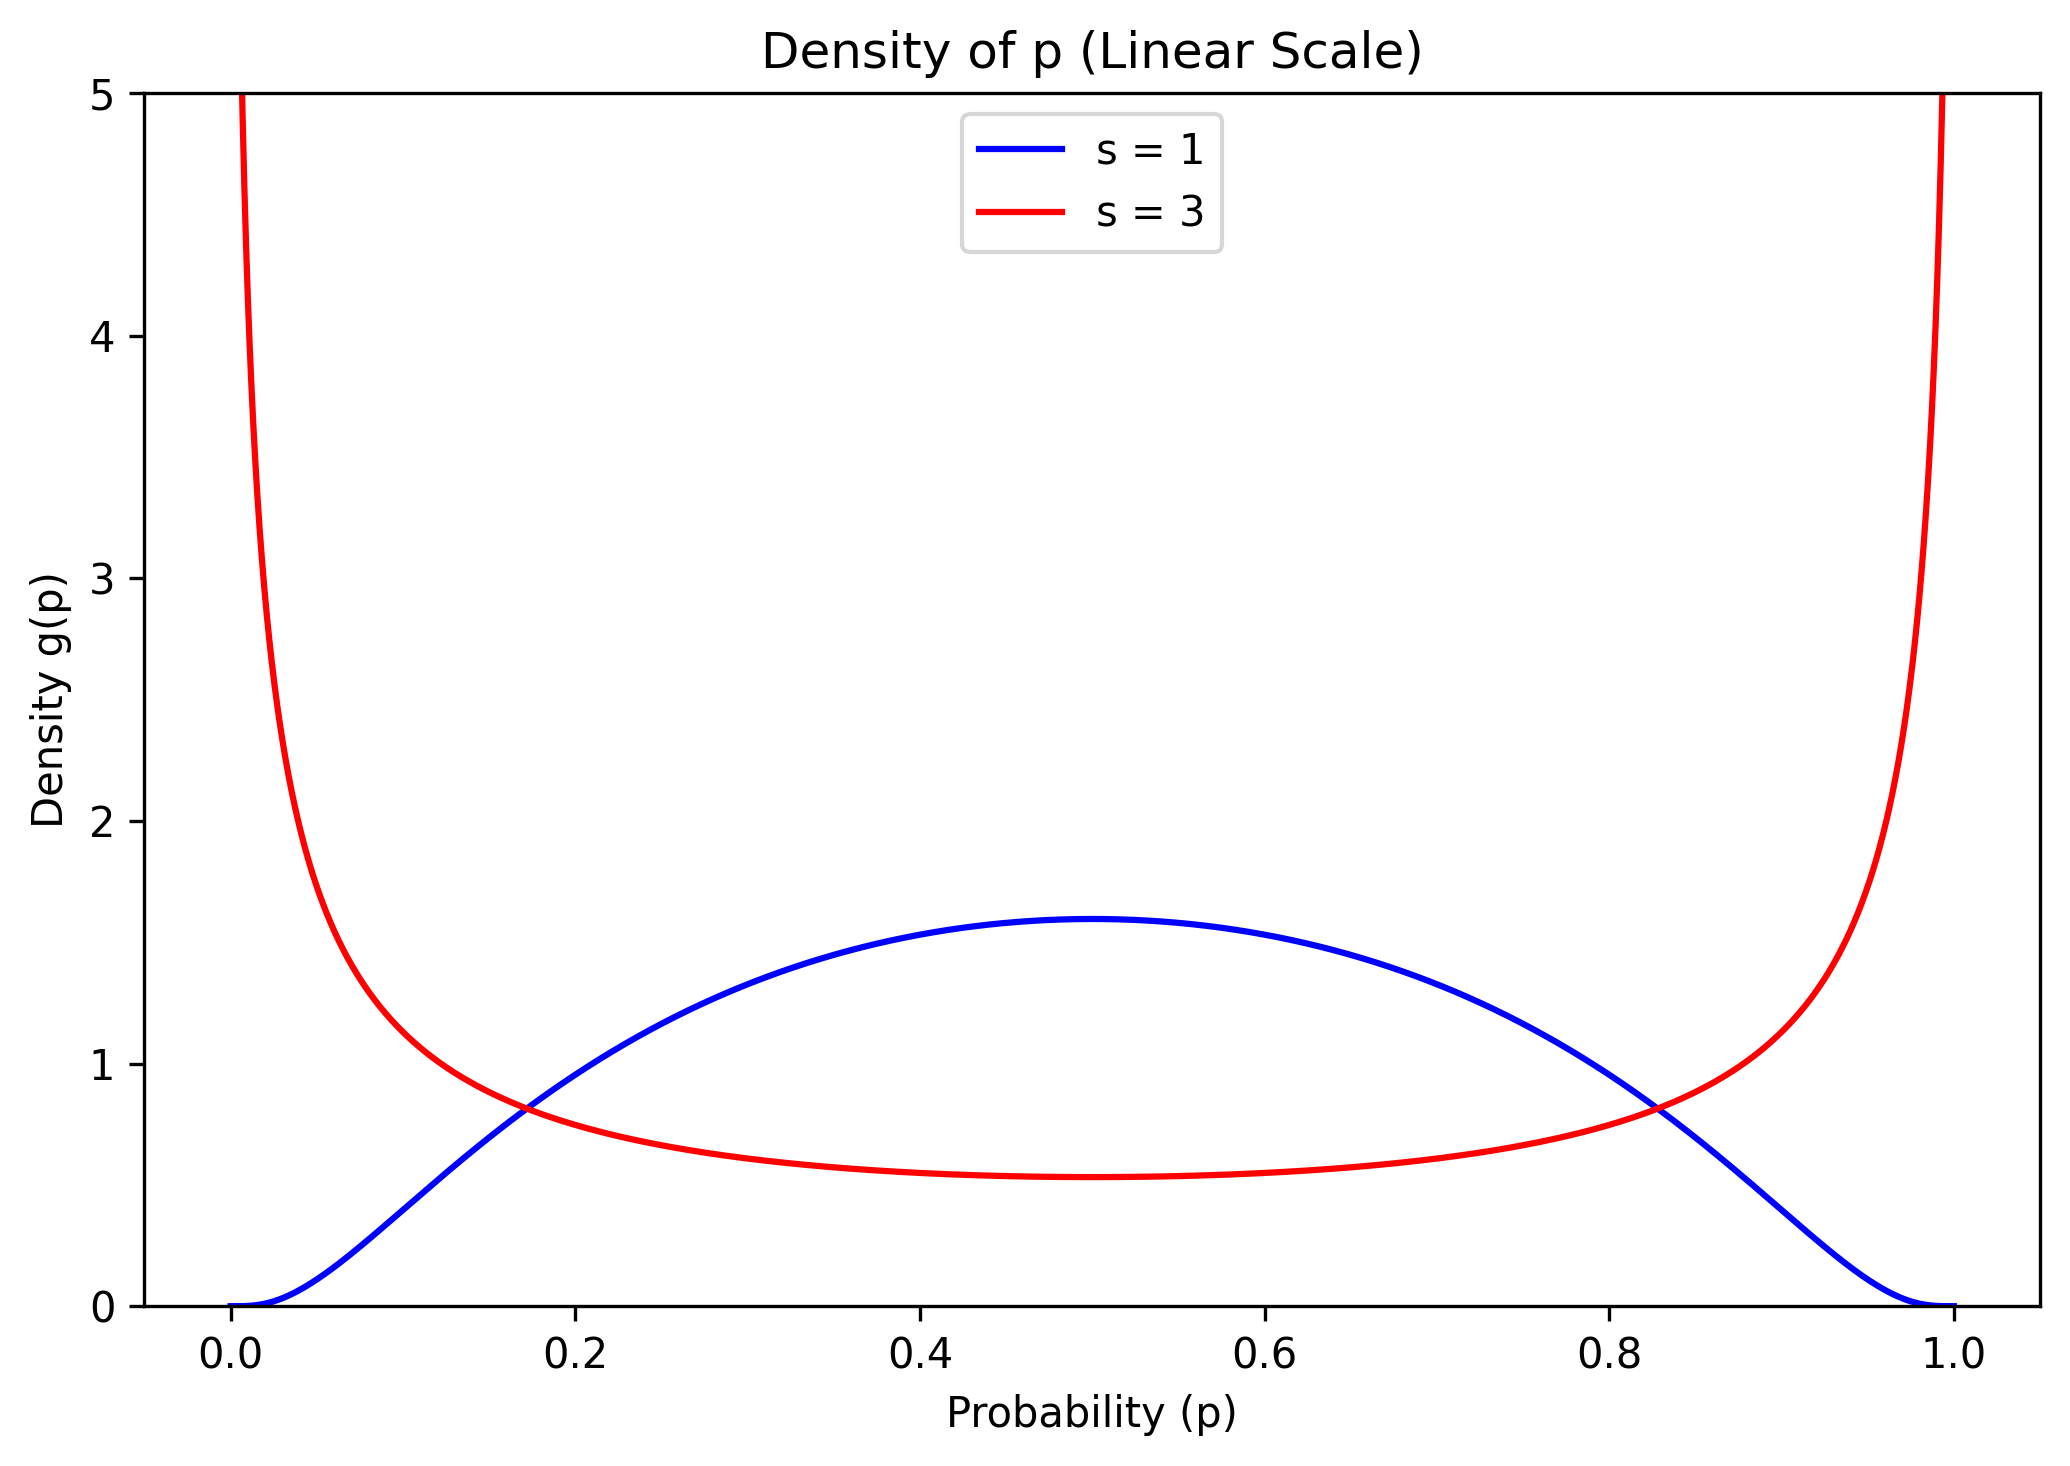
\includegraphics[width=0.5\linewidth]{p6c.png}
\end{figure}
This plot shows how the idea that a large prior standard deviation on the log-odds is actually informative. When $s=1$, the probability mass is centered which implies the probability lies in the middle. When $s=3$, we get a U-shaped density curve (due to the $|dx/dy|$ transformation pushing the prob mass at the extreme ends) which implies that we're very certain that the probability is either 0 or 1.
}

d. (4 points) Now consider the inverse problem.  We observe that some monotone increasing function $z=\phi(a)$ of the same standard normal $a$ is uniformly distributed on $(0,1)$.  Use the transformation law to find $\phi$, and explain how this result relates to the inverse transformation method for sampling.

\textcolor{red}{
If its uniformly distributed on $(0,1)$, that must mean $g(z)=1=f(a) \vert{} \frac{da}{dz} \vert{}$.  $\phi$ is monotone increasing so $\frac{da}{dz}$ doesn't need absolute bars. Thus, $1=f(a)\frac{da}{dz} \rightarrow dz = f(a)da$. Integrating shows that $z$ is the integral of the PDF $f(a)$ which means its its CDF. Thus, $\phi(a)$ is the CDF of a standard normal distribution. What this means is that if you plug any random variable into its own CDF, the output is uniform on $(0,1)$. The inverse CDF method  involves drawing some random number $x \sim \text{Uniform}(0, 1)$ then finding a target value by calculating the inverse of the CDF at that uniform point. Passing a standard nromal varaible through its own CDF flattens it into $\text{Uniform}(0, 1)$, taking a $\text{Uniform}(0, 1)$ random draw and passing it through the inverse CDF reverts to a standard bell curve.
}

\end{document}
